% corrected LN 87

\subsection{Assessment}
\subsubsection{NFR01: Performance evaluation}~\label{assessment}~\\

In this section, the performance of the four ANNs investigated in
Section~\ref{ann} are evaluated. We use the English and Luxembourgish dataset
for the performance analysis.\\

The English and Luxembourgish dataset contains spoken words $w \in
\{'0',\dots,'9'\}$. The English dataset consists of 17749 data instances whereas
the Luxembourgish consists of 500 data instances.\\

The first step is to choose an optimal optimizer. The choice is between using
the stochastic gradient descent (SGD) or Adam optimizer. The latter is a
combination of two extensions of SGD, Adaptive Gradient Algorithm (AdaGrad) and
Root Mean Square Propagation (RMSProp)~\cite{Adam}. The four models will be
trained on the English dataset to designate the right optimizer and number of
epochs. Their training will be visualized with $60\ epochs$ each. The training
visualization is in the appendix as follows:\\

\begin{enumerate}[label=\arabic*.]
  \item Feedforward
    \begin{itemize}
      \item Validation accuracy in Figure.\ref{ffa}
      \item Validation loss in Figure.\ref{ffl}
    \end{itemize}
  \item RNN
    \begin{itemize}
      \item Validation accuracy in Figure.\ref{rnna}
      \item Validation loss in Figure.\ref{rnnl}
    \end{itemize}
  \item LSTM
    \begin{itemize}
      \item Validation accuracy in Figure.\ref{lstma}
      \item Validation loss in Figure.\ref{lstml}
    \end{itemize}
  \item GRU
    \begin{itemize}
      \item Validation accuracy in Figure.\ref{grua}
      \item Validation loss in Figure.\ref{grul}
    \end{itemize}
\end{enumerate}~\\

Let $n=60$ for the number of epochs. The two optimizers return the following
testing accuracies (acc) and losses:

\begin{table}[H]
    \centering
    \resizebox{\columnwidth}{!}{%
    \begin{tabular}{|c|c|c|c|c|c|c|c|c|}
        \hline
        \multirow{2}{*}{Optimizer} & \multicolumn{2}{c|}{FF} &
        \multicolumn{2}{c|}{RNN} & \multicolumn{2}{c|}{LSTM} &
        \multicolumn{2}{c|}{GRU} \\
        \cline{2-9}
        & {acc} & {loss} & {acc} & {loss} & {acc} & {loss} & {acc} & {loss}\\
        \hline
        SGD & 0.79 & 0.65 & 0.43 & 1.51 & 0.86 & 0.46 & 0.85 & 0.46 \\ \hline
        Adam & 0.87 & 0.47 & 0.72 & 0.97 & 0.94 & 0.24 & 0.94 & 0.24 \\ \hline
    \end{tabular}%
    \caption{Comparison of the four models' testing results using SGD and Adam.
    The models were trained on the English dataset.}
    \label{table:comparison}
    }
\end{table}

Tabel~\ref{table:comparison} shows the validation accuracies using the Adam
optimizer yield better accuracies compared to SGD. For the following
investigation, the Adam optimizer is considered.\\

The next step is to choose the number of epochs which will be used for the
performance analysis. The graphs show the loss converges around $40$ epochs.
Therefore, we choose $epochs = 40$.\\

Let $epochs = 40$ to evaluate each model's performance, we have:

\begin{table}[H]
    \centering
    \resizebox{\columnwidth}{!}{%
    \begin{tabular}{|c|c|c|c|c|c|c|c|c|}
        \hline
        \multirow{2}{*}{Optimizer} & \multicolumn{2}{c|}{FF} &
        \multicolumn{2}{c|}{RNN} & \multicolumn{2}{c|}{LSTM} &
        \multicolumn{2}{c|}{GRU} \\
        \cline{2-9}
                                 & {acc} & {loss} & {acc} & {loss} & {acc} &
        {loss} & {acc} & {loss}\\ \hline
        Adam & 0.83 & 0.54 & 0.63 & 1.10 & 0.937 & 0.23 & 0.94 &
        0.23 \\ \hline
    \end{tabular}%
    \caption{The testing results of the four models using Adam. The four models
    were trained on the English dataset. $FF$ is the abbreviation for feedforward
    and $acc$ stands for accuracy.}
    \label{table:40}
    }
\end{table}

Inspecting the results shows that LSTM and GRU perform better than feedforward
and RNN. The overall performance is slightly underneath the performance at 60
epochs. In this case, RNN has the lowest accuracy. This can be explained with
the vanishing and exploding gradients or because the learning rate was not set
optimally during training. As expected, LSTM and GRU perform better than RNN
since they deal with the challenge of long-term dependencies. Compared to
feedforward, LSTM and GRU have better accuracy since they take advantage of
their recurrent units to process series data.\\

\textbf{Training on Luxembourgish dataset.} The same models used to train on the
English dataset were used to train on the Luxembourgish dataset. The following
testing accuracies and losses were obtained while training on the Luxembourgish
dataset:

\begin{table}[H]
    \centering
    \resizebox{\columnwidth}{!}{%
    \begin{tabular}{|c|c|c|c|c|c|c|c|c|}
        \hline
        \multirow{2}{*}{Optimizer} & \multicolumn{2}{c|}{FF} &
        \multicolumn{2}{c|}{RNN} & \multicolumn{2}{c|}{LSTM} &
        \multicolumn{2}{c|}{GRU} \\
        \cline{2-9}
        & {acc} & {loss} & {acc} & {loss} & {acc} & {loss} & {acc} & {loss}\\
        \hline
        Adam & 0.84 & 0.59 & 0.73 & 0.83 & 1.0 & 0.02 & 0.99 & 0.02 \\ \hline
    \end{tabular}%
    \caption{The testing results of the four models using Adam. The four models
    were trained on the Luxembourgish dataset. The dataset contains 50 instances
    of each spoken word. FF is the abbreviation for feedforward and $acc$ stands for
    accuracy.}
    \label{table:lux}
    }
\end{table}

The results show that LSTM and GRU generalize better than feedforward and RNN.
LSTM and GRU are outperforming RNN in these results as well. The validation
accuracies of LSTM and GRU are both roughly 0.99\%. The high accuracy of LSTM
and GRU can be explained by the small dataset which is also speaker-dependent.
The results of LSTM and GRU will drop if the dataset grows and contains a
variety of speakers.\\

\begin{figure}[h]
  \centering
  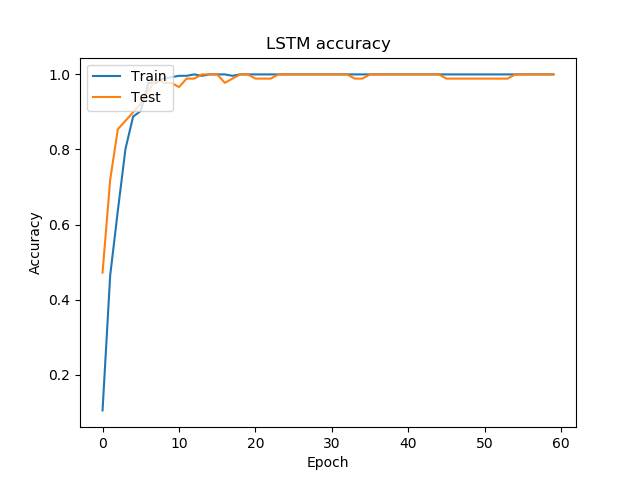
\includegraphics[scale=0.5]{luxlstma.png}
  \caption{Training and validation accuracy of LSTM model trained on
  Luxembourgish dataset.}
\end{figure}

\begin{figure}[h]
  \centering
  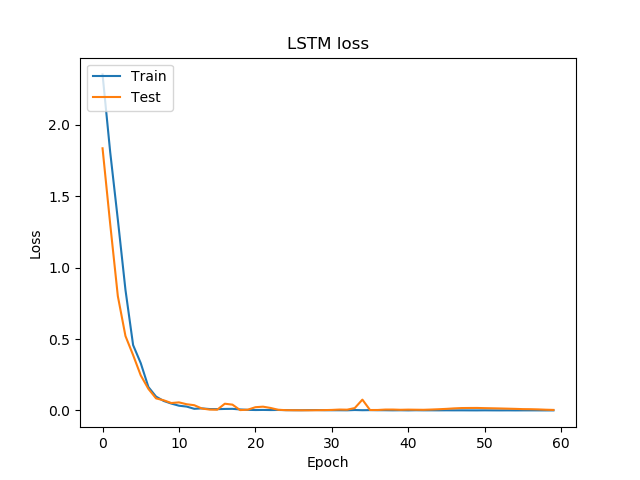
\includegraphics[scale=0.5]{luxlstml.png}
  \caption{Training and validation loss of LSTM model trained on Luxembourgish
  dadataset.}
\end{figure}

\begin{figure}[h]
  \centering
  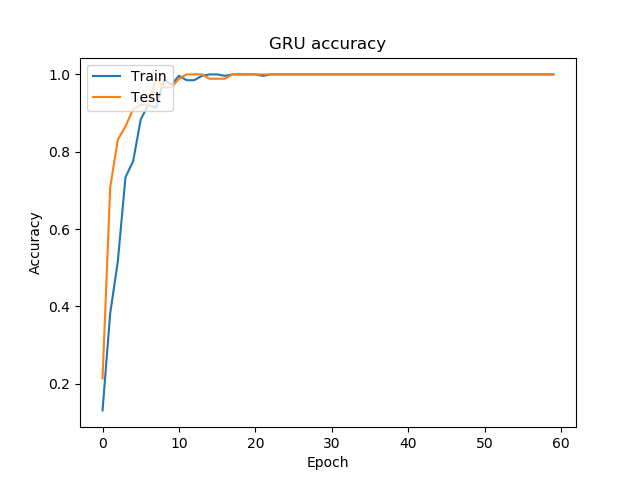
\includegraphics[scale=0.5]{luxgrua.png}
  \caption{Training and validation accuracy of GRU model trained on Luxembourgish
  dadataset.}
\end{figure}

\begin{figure}[h]
  \centering
  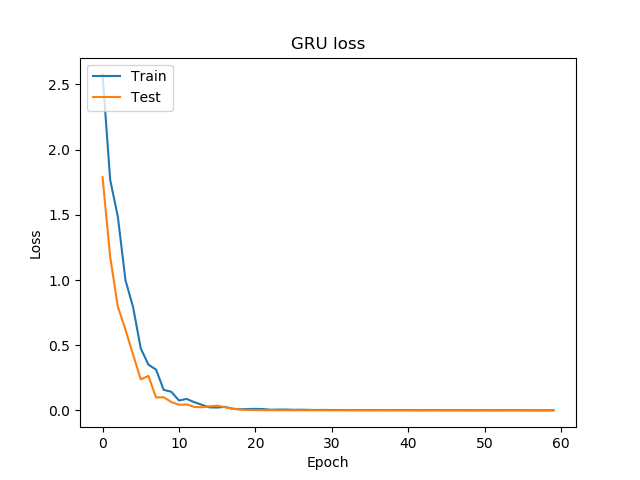
\includegraphics[scale=0.5]{luxgrul.png}
  \caption{Training and validation loss of GRU model trained on Luxembourgish
  dadataset.}
\end{figure}
